\chapter{Dataset}
\label{ch:dataset}
This chapter discusses the dataset used in our work. We use the \gls{scid} dataset \cite{ni_esim_2017}\footnote{The dataset can be downloaded here: https://eezkni.github.io/publications/ESIM.html.}.
The important characteristics of the dataset are text content on screenshots, different distortion levels and \gls{mos} values for each image. This combination is difficult to find.

\section{Overview}
\label{sec:dataset_overview}
An overview of the 40 reference images of the dataset can be seen in \autoref{fig:dataset_overview}.

\begin{figure}[h]
    \centering
    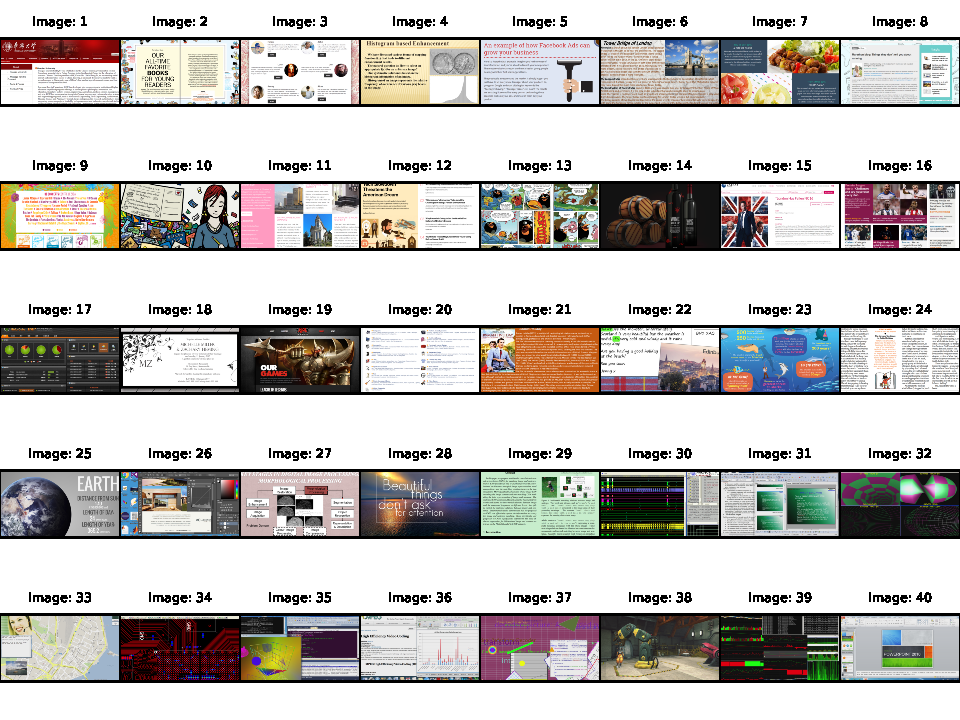
\includegraphics[width=\textwidth]{reference_images}
    \caption{Overview of the dataset.}
    \label{fig:dataset_overview}
\end{figure}

Additionally, the dataset contains 1800 distorted images.
They are distorted with 9 different distortion types, each with 5 different distortion levels.

\section{Distortion types}
\label{sec:dataset_distortion_types}

In this section we will discuss the different distortion types used in the dataset.
The nine different distortion types can be seen in \autoref{fig:distortion_types}, applied to the image in \autoref{fig:img29}.

\begin{figure}[h]
    \centering
    \begin{subfigure}[b]{0.3\textwidth}
        \includegraphics[width=\textwidth]{../../data/raw/scid/DistortedSCIs/SCI29_1_5.png}
        \caption{Gaussian Noise}
        \label{fig:distortion_type_1}
    \end{subfigure}
    \hfill
    \begin{subfigure}[b]{0.3\textwidth}
        \includegraphics[width=\textwidth]{../../data/raw/scid/DistortedSCIs/SCI29_2_5.png}
        \caption{Gaussian Blur}
        \label{fig:distortion_type_2}
    \end{subfigure}
    \hfill
    \begin{subfigure}[b]{0.3\textwidth}
        \includegraphics[width=\textwidth]{../../data/raw/scid/DistortedSCIs/SCI29_3_5.png}
        \caption{Motion Blur}
        \label{fig:distortion_type_3}
    \end{subfigure}
    \newline
    \begin{subfigure}[b]{0.3\textwidth}
        \includegraphics[width=\textwidth]{../../data/raw/scid/DistortedSCIs/SCI29_4_5.png}
        \caption{Contrast Change}
        \label{fig:distortion_type_4}
    \end{subfigure}
    \hfill
    \begin{subfigure}[b]{0.3\textwidth}
        \includegraphics[width=\textwidth]{../../data/raw/scid/DistortedSCIs/SCI29_5_5.png}
        \caption{JPEG Compression}
        \label{fig:distortion_type_5}
    \end{subfigure}
    \hfill
    \begin{subfigure}[b]{0.3\textwidth}
        \includegraphics[width=\textwidth]{../../data/raw/scid/DistortedSCIs/SCI29_6_5.png}
        \caption{JPEG2000 Compression}
        \label{fig:distortion_type_6}
    \end{subfigure}
    \newline
    \begin{subfigure}[b]{0.3\textwidth}
        \includegraphics[width=\textwidth]{../../data/raw/scid/DistortedSCIs/SCI29_7_5.png}
        \caption{Color Saturation Change}
        \label{fig:distortion_type_7}
    \end{subfigure}
    \hfill
    \begin{subfigure}[b]{0.3\textwidth}
        \includegraphics[width=\textwidth]{../../data/raw/scid/DistortedSCIs/SCI29_8_5.png}
        \caption{HEVC Screen Content Coding}
        \label{fig:distortion_type_8}
    \end{subfigure}
    \hfill
    \begin{subfigure}[b]{0.3\textwidth}
        \includegraphics[width=\textwidth]{../../data/raw/scid/DistortedSCIs/SCI29_9_5.png}
        \caption{Color Quantization with dithering}
        \label{fig:distortion_type_9}
    \end{subfigure}
    \caption{Distorted image 29 with 9 different distortion types and distortion level 5.}
    \label{fig:distortion_types}
\end{figure}

We can see, that the different distortion types have different effects on the text in the image.
Distortions like the contrast change don't affect the text much.
However, Gaussian noise or blur can make the text unreadable.

\section{Labeling}
\label{sec:dataset_labeling}

The dataset doesn't have any text labels.
Thus we labeled the dataset ourselves.
We typed the text on each image into a text file, starting on the top left and ending on the bottom right.
Our order of labeling was always dependent on the top left corner of a text element.
Thus if two paragraphs were side by side we always labeled the first line of the left paragraph first, then the first line of the right paragraph, then the second line of the left paragraph and so on.
This way we could ensure that we have a unifying representation of the text with regards to the two /gls{ocr} algorithms we used.
The algorithms have different modes for combining text elements, and thus produce differently connected paragraphs, if using the paragraph option.
To get a generalized result we use the option of raw text detection and text recognition to get the bounding boxes and the text.
We then use the bounding boxes to get the text in the correct order.

In \autoref{fig:ref29} we can see that it is sometimes difficult to say which text element is higher than another, especially if the text elements have different font sizes.
Thus we decided against using one of the \gls{ocr} algorithms to predict the text and then correct it to create the ground truth, to not introduce bias towards one of the algorithms with regard to the positions of the text elements.
We used the images, a ruler and our eyes to determine the correct order of the text elements.

\begin{figure}
    \centering
    \includegraphics[width=\textwidth]{../../data/raw/scid/ReferenceSCIs/SCI29.png}
    \caption{Reference image 29.}
    \label{fig:ref29}
\end{figure}

\section{Analysis}
\label{sec:dataset_analysis}

In \autoref{fig:cer_vs_mos} the cer is plotted against the MOS.
It shows the \gls{cer} and \gls{mos} of all 1800 distorted images compared to their reference image.

\begin{figure}[h]
    \centering
    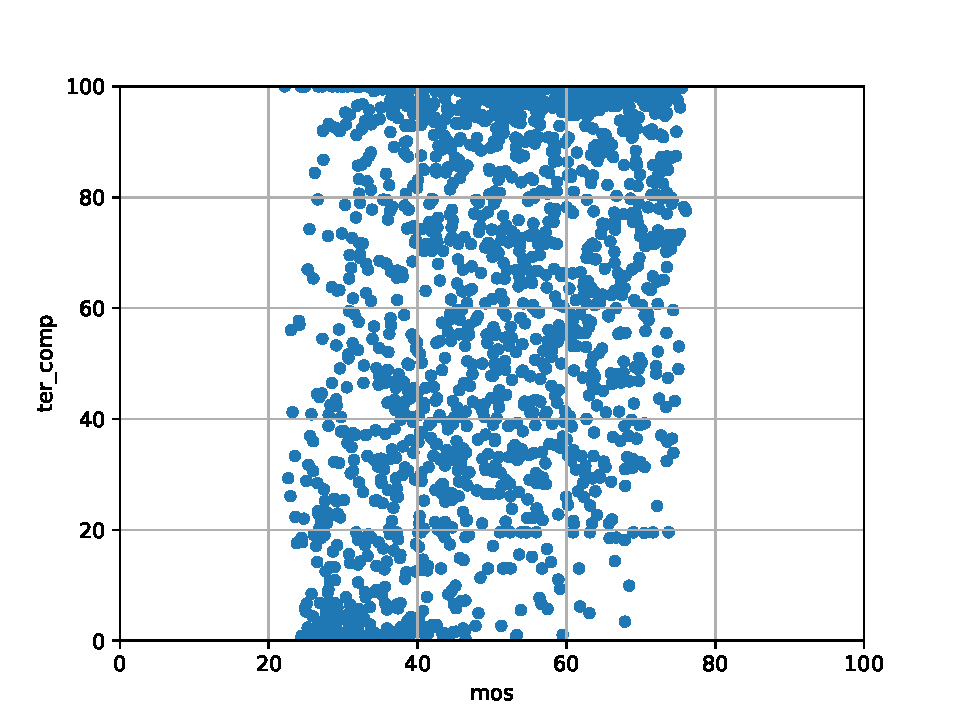
\includegraphics[width=\textwidth]{mosvster_all}
    \caption{\gls{cer} of all distorted images compared to their reference image plotted against the \gls{mos}.}
    \label{fig:cer_vs_mos}
\end{figure}

In \autoref{fig:cer_vs_mos_456} the \gls{cer} is plotted against the \gls{mos}.
We are only using a selection of images in this plot.
These images (SCI4, SCI5, SCI6, SCI22 and SCI29) have their main focus on text, and have simple text structure.
\begin{figure}[h]
    \centering
    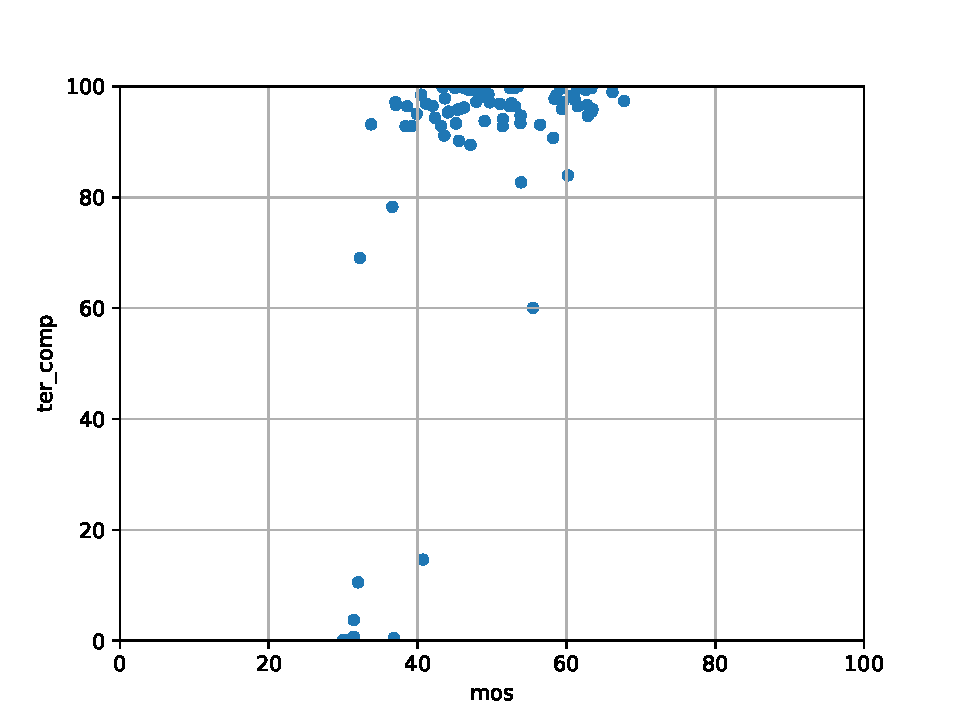
\includegraphics[width=\textwidth]{mosvster__456_22_29__1_4}
    \caption{\gls{cer} of a selection of distorted images compared to their reference image.}
    \label{fig:cer_vs_mos_456}
\end{figure}
